\newpage\part{Flash Cards}

\section{Farmaci del SNC e del SNP}

\begin{tikzpicture}
	\tikzset{level distance=85pt,frontier/.style={distance from root=350pt}} 
	\Tree
	[.SNC
		[.Periferico
			[.Sensitivo ]
			[.Autonomo
		 		[ .{Simpatico\\ (toraco--addominale)} {gangli pre e para--vertebrali} ]
				[ .{Parasimpatico \\(nervi crani e sacrale)} {nell'intima degli organi} ]
			]
			[.Gastroenterico {plessi mioenterici (Auerbach) e\\ sottomucosi (Meissner)}
			]
		]
		[.Centrale ]
	]
\end{tikzpicture}

L'adrenalina è un ormone. Noradrenalina è un neurotrasmettitore

\begin{tikzpicture}
	\tikzset{level 1/.style={level distance=150pt}}
	\Tree
	[.{Neurotrasmettitori\\ SNP}
		 [.\node(acetilcolina){acetilcolina}; {recettori colinergici} ]
		 [.{noradrenalina\\ (monoammina)} {recettori adrenergici} ]
		 [.\node(serotonina){serotonina\\5-HT 5-idrossitriptamina\\ (monoammina)}; {recettori serotoninergici} ]
		 [.{monossido d'azoto (NO)} ] 
		 [.purine ]
	]
	\begin{scope}[yshift=-11em]
	\Tree
	[.\node(snc){Neurotrasmettitori\\ SNC};
		[.{dopamina\\ (monoammina)} {recettori dopaminergici} ]
		[.{aminoacidi eccitatori}
			L--glutammato
			aspatato
			omocisteinato
		]
		[.{aminoacidi inibitori}
			GABA
			glicina
		]
	]
	\end{scope}
	\draw[drawarrow] (snc.east) to[in=180,out=40] (acetilcolina.west)
		(snc.east) to[in=180,out=0] (serotonina.west);
\end{tikzpicture}

\begin{tikzpicture}
	\Tree
	[.{Siti di azione\\ farmaci del SNC}
		[.{fibra pre--sinapica}
			{sintesi}
			{immagazzinamento}
			{rilascio}
			{ricaptazione}
			{metabolismo}
		]
		[.{fessura sinaptica}
			{recettore}
			{degradazione}
		]
		[.{fibra post--sinapica}
			{conducibilità ionica\\ del canale}
			{segnalazione retrograda}
		]
	]
\end{tikzpicture}

\begin{tikzpicture}
\tikzset{level 2/.style={level distance=130pt}}
	\Tree
	[.{Distribuzione\\ dei recettori}
		[. {pre--gangliari\\ para e orto}
			{tutte colinergiche con rec. nicotinico}
		]
		[. {parasimpatico \\ post gangliare}
			{colinergiche con rec. muscarinico}
		]
		[. Simpatico
			{quasi tutto adrenergico}
			[. {muscolatura liscia rene}
				dopaminergica
			]
			[. {gh. sudoripare}
				{colinergiche con rec. muscarinico}
			]
		]
		[. {midollare surrene}
			{libera adrenalina e noradrenalina in circolo}
		]
	]
\end{tikzpicture}


\subsection{Acetilcolina}


\begin{tikzpicture}
	\tikzset{level 1/.style={level distance=150pt}}
	\Tree
	[.\node(loc){localizzazione}; {tutte le fibre pregangliali sia para che orto\\ nicotiniche} {parasimpatiche post gangliali (quasi tutte).\\ muscariniche} {ghiandole sudoripare (simpatico)\\ muscariniche} {giunzione neuromuscolare\\ nicotiniche} 
		[.SNC
			proencefalo
			mesencefalo
			{tronco celebrale}
			cervelletto
			{interneuroni corpo striato}
		]
	]
\end{tikzpicture}

\begin{tikzpicture}
	\tikzset{level 2/.style={level distance=130pt}, level 3/.style={level distance=120pt}}
	\Tree
	[.Sintesi
		[.colina \edge node[smallfont,yshift=5pt,xshift=5.4em]{entra nel neurone} node[smallfont,yshift=-5pt,xshift=5.4em]{tappa limitante};
			[.{acetilCOA + colina} \edge node[smallfont,yshift=-5pt,xshift=5em]{acetiltrasferasi} node[smallfont,yshift=5pt,xshift=5em]{colina}; acetilcolina ]
		]
	]
\end{tikzpicture}

\begin{tikzpicture}
	\tikzset{level 2/.style={level distance=130pt}}
	\Tree
	[.Degradazione
		[.acetilcolina \edge node[smallfont, yshift=-5pt,xshift=5.3em]{acetilcolinesterasi}; {acetato + colina} ]
	]
\end{tikzpicture}

L'acetil--COA è sintetizzato nei mitocondri del neurone

La colina entra nel neurone tramite un trasportatore detto CHT in simporto con il sodio. Questo trasportatore è bloccato da farmaci sperimentali chiamati emicolini.

\begin{nicebox}{VAMP}
Proteine di membrana associate alle vescicole
\end{nicebox}

\begin{tikzpicture}
	\Tree
	[.Liberazione 
		[.{Ca${}^{2+}$ + VAMP/SNAPS}
			[.{fusione vescicole con\\ membrana neuronale} esocitosi
			]
		]
	]
\end{tikzpicture}

\begin{tikzpicture}
\begin{scope}[scale=0.3]
	\tikzstyle{arrow}=[latex-,draw=black,line width=1.500]
	\tikzstyle{arrow1}=[-latex,draw=black,line width=1.500]
	\tikzstyle{none}=[inner sep=0pt]
		\node [style=none] (0) at (-7, -2) {};
		\node [style=none] (1) at (-7, 1) {};
		\node [style=none] (2) at (-3, -2) {};
		\node [style=none] (3) at (-3, 1) {};
		\node [style=none] (4) at (2.5, 0.75) {};
		\node [style=none] (5) at (-12, 1) {};
		\node [style=none] (6) at (-14, -1) {};
		\node [style=none] (7) at (4, -3.5) {};
		\node [style=none] (8) at (-10.75, -2.5) {\tiny VAT: Trasportatore associato vescicole (antiporto Ach-$H^+$)};
		\node [style=none] (9) at (-5, 0.25) {};
		\node [style=none] (10) at (-5, -1.5) {};
		\node [style=none] (11) at (-5, 0.25) {};
		\node [style=none] (12) at (-3.250001, 5) {};
		\node [style=none] (13) at (-3.250001, -6.75) {};
		\node [style=none] (14) at (-1, 3.25) {\tiny \bf Vescicola};
		\node [style=none] (15) at (-10.5, 1.75) {\tiny $H^+$};
		\node [style=none] (16) at (-12, -1.5) {\tiny Ach};
		\draw [bend left, looseness=1.00] (0.center) to (2.center);
		\draw [bend right, looseness=1.25] (1.center) to (3.center);
		\draw [style=arrow, bend right=15, looseness=1.00] (5.center) to (4.center);
		\draw [style=arrow1, in=157, out=7, looseness=1.00] (6.center) to (7.center);
		\draw [bend left=15, looseness=0.75] (9.center) to (12.center);
		\draw [bend right=15, looseness=1.00] (10.center) to (13.center);

\end{scope}

\begin{scope}[xshift=100pt, yshift=-50pt]
	\tikzstyle{cwhite}=[circle,shadedraw=yellow];
	\shade[ball color=yellow] node (ach) {\small Ach} circle[radius=.45];
	\draw (ach) -- +(.7,.7) node(vamp){} arc [start angle=225, end angle=270, radius=6pt]  (.7,.7) arc [start angle=225, end angle=180, radius=6pt];
	\draw (2,2) arc [start angle=45, end angle=0, radius=3cm] node[midway,above,sloped]{\tiny spazio sinaptico} ;
	\draw (2,2) 
		arc [start angle=45, end angle=60, radius=3cm] node(a){} 
		node[above right=2pt and 2pt of a] {\tiny Canale Ca${}^{2+}$}
		(a) arc [start angle=140, end angle=120, radius=1cm]
		(a) arc [start angle=140, end angle=160, radius=1cm];
	\path (2,2) arc [start angle=45, end angle=65, radius=3cm] node(b){};
	\draw (b) arc [start angle=-50, end angle=-30, radius=1cm]
		(b) arc [start angle=-50, end angle=-70, radius=1cm]
		(b) arc [start angle=65, end angle=80, radius=3cm];
	\draw (2,2) -- (1.3,1.3);
	\filldraw (1.3,1.3) circle[radius=3pt] node(snap){};
	\draw[->, shorten <=0pt,shorten >=2pt] (vamp)--(snap) node[midway,above,circle,draw,,yshift=3pt,xshift=-8pt]{\tiny 2};
	\draw[->, shorten <=0pt,shorten >=2pt] (ach) to[out=-20,in=225] node[midway,below,circle,draw,yshift=-5pt]{\tiny 3}  (4,1) ;
	\draw[->, shorten <=2pt,shorten >=6pt](3,3.5) to[out=205,in=90] node[near end,above,circle,draw,yshift=15pt]{\tiny 1}  node[very near end,above,yshift=15pt,xshift=-2pt]{\tiny Ca${}^{2+}$} (ach) ;
	\node at (1,.4) {\tiny VAMP};
	\node at (1.9,1.3) {\tiny SNAP};
	\end{scope}
\end{tikzpicture}

Tossina botulinica altera alcuni amminoacidi di vAMP e sNAP impedendo il rilascio della vescicola

\begin{tikzpicture}
	\tikzset{level distance=75pt}
	\Tree
	[.Effetti
		[.SNP
			[.{$\uparrow$permeabilità\\ Na${}^+$, Ca${}^{2+}$}
				[.depolarizzazione
					[.{fibre post gangliari} PdA ]
					[.{fibre muscolari} {generazione\\ potenziale\\ di placca}
					]
				]
			]
		]
		[.SNC
			[.{$\uparrow$Ach}
				{veglia,\\ apprendimento,\\ memoria}
			]
		]
	]
\end{tikzpicture}

\begin{tikzpicture}
	\tikzset{level 1/.style={level distance=100pt},level 2/.style={level distance=110pt},level 3/.style={level distance=140pt}}
	\Tree
	[.{Recettore colinergico}
		[.{muscarinico\\ (metabotropo)}
			[.{M${}_1$ eccitatorio\\ $\uparrow\text{IP}_3, \uparrow\text{DAG},\uparrow\text{Ca}^{2+}$} {SNC, simpatico post--gangliare,\\ cellule parietali dello stomaco}
			]
			[.{M${}_2$ inibitorio $\downarrow$cAMP } {cuore, endotelio dei vasi\\ muscolo liscio}
			]
			[.{M${}_3$ come $\text{M}_1$} {ghiandole esocrine, endotelio dei vasi\\ occhio, polmone, intestino}
			]
			[.{M${}_4$ come $\text{M}_2$} {SNC}
			]
			[.{M${}_5$  come $\text{M}_1$} {endotelio vasale del cervello,\\ SNC (facilita rilascio\\ glutammato e dopamina)}
			]
		]
		[.{nicotinico\\ (ionotropo)\\ apertura canali \ce{Na+}, \ce{K+}\\ con depolarizzazione}
			[.{N${}_\text{N}$ gangliare} {para e ortosimpatico gangliare} ]
			[.{N${}_\text{M}$ muscolare} {giunzione\\ neuromuscolare} ]
		]
	]
\end{tikzpicture}

Per il recettore nicotinico, c'è bisogno di due molecole di agonista per attivare il recettore

\begin{tikzpicture}
	\tikzset{level distance=90pt}
	\Tree
	[.{Farmacologia\\ dell'occhio}
		[.{Muscolo circolare}
			[. {Costrittore pupilla}
				[. \ce{M3} 
					miosi
				]
			]
		]
		[.{Muscolo ciliare}
			[. {Accomodazione fuoco}
				[. \ce{M3} 
					Accomodazione
					{apertura pori\\ efflusso umor acqueo}
				]
				[. $\beta_2$ ]
			]
		]
		[.{Muscolo radiale}
			[. {dilatatore pupilla}
				[. $\alpha_1$ 
					midriasi
				]
			]
		]
		[.{Epitelio ciliare}
			[. {secrezione umore acqueo}
				$\beta$
			]
		]
	]
\end{tikzpicture}

Glaucoma: colinergici + $\beta$--bloccanti

Atropina (antagonista colinergico): visite oculistiche, \dwa secrezione lacrimale

\subsubsection{Agonisti colinergici}

\begin{tikzpicture}
	\begin{scope}
	\tikzset{
		level distance=80pt,
		level 1/.style={level distance=70pt},
		level 2/.style={level distance=70pt},
		frontier/.style={distance from root=400pt} 
	}
	\Tree
	[.\node(main){Tipo}; 
		[.diretti
			[.{attivano recettori} 
				[.{esteri della colina} 
					[. {muscarinici\\ nicoticini\\ \amminaq}
						\node(ach){acetilcolina };
						metacolina
						carbacolo
						\node[farmaco](beta){\index{betanecolo}betanecolo};
					]
				]
				[.alcaloidi
					[.muscarinici
						{muscarina \amminaq\\(fungo)}
						\node[farmaco]{\index{pilocarpina}pilocarpina \amminat};
					]
					[.nitotinici \node[farmaco]{\index{nicotina}nicotina \amminat}; ]				
				]
			]
		]
		[.indiretti
			[.\node(AchEI){inibitori AchE}; 
			]
		]
	]	
	\node[right=5pt of ach] (achn) {};
	\node[right=5pt of beta] (betan) {};
	\draw[drawarrow] (achn) -- (betan) node[midway,above,sloped] {\tiny $\uparrow$resist. idrolisi e quindi durata azione};
\end{scope}
\begin{scope}[yshift=-14em]
	\Tree
	[.\node(AchEIa){inibitori AchE};
		[.{alcool + \amminaq }
			[.\node[farmaco]{\index{edrofonio}edrofonio}; 
				[.{legame idrogeno\\ o ionico con AchE} {idrolisi in minuti}
				]
			]
		]
		[.carbammati 
			[.\node[farmaco]{\index{neostigmina}neostigmina \amminaq\\ \index{fisostigmina}fisostigmina\footnotemark\amminat}; 
				[.{legame covalente con AchE} {idrolisi in ore}
				]
			]
		]
		[.organofosfati
			[.\node[farmaco](ecotiopato){\index{ecotiopato}ecotiopato\footnotemark\amminaq};
				[.\node(fAchE){fosforilazione AchE}; \node(idro){idrolisi in giorni};
				]
			]
			\node(somar){somar\\ (gas nervino)};
		]
	]		
	\draw[drawarrow] (somar) to[out=0,in=180] (fAchE);
	\node[chartnode,below=1em of fAchE] (invec) {invecchiamento\\rottura legame O-P\\ con raffozamento\\ legame con AchE}; 
	\node[chartnode,below=1em of idro] (pral) {pralidossima pu\`o\\ scindere la\\ fosforilazione};
	\draw[drawarrow] (pral)--(fAchE) node[midway,above,sloped] {\tiny qui si};
	\draw[drawarrow] (pral)--(invec) node[midway,above,sloped] {\tiny qui no};
	\node[below right=8pt and 5pt of somar] (somary) {};
	\node[above=9em of somary] (neox) {};
	\draw[drawarrow] (neox) -- (somary) node[midway,above,sloped] {\tiny $\uparrow$durata azione};
	\draw[drawarrow] (AchEI.south) to[out=-90,in=90] (AchEIa);
\end{scope}
\end{tikzpicture}

Nota: Mettere da qualche parte il tacrida (si usa nell'Alzheimer) che è un inibitore della colinesterasi che poi si ritrova come inibitori del citocromo P450.

Gli \amminaq hanno scarso assorbimento

\footnotetext{Presente nella fava del Calabar}
\footnotetext{Unico degli organofosfati ad essere un ammina quateraria e quindi altamente polare e pu\`o essere preparato come soluzione acquosa. Era utilizzato per il glaucoma, ora in disuso.}

\begin{tikzpicture}
	\tikzset{level distance=120pt, level 2/.style={level distance=150pt}}
	\Tree
	[.\node(sub){Effetti}; 
		[.{SNC ($\text M_1$)} {tremore, ipotermina, $\uparrow$capacità cognittive (a)}	
		]
		[.{occhio ($\text M_3$)}
			{costrizione muscolo circolare (miosi)\\ contrazione muscolo ciliare (accomodamento da vicino)\\ facilitazione nel deflusso dell'umor acqueo}
		]
		[.{cuore ($\text M_2$)}
			{\upa\ce{I_k} $\downarrow$frequenza (cronotopo-), \dwa\ce{I_{Ca}} $\downarrow$forza (inotropo-),\\ \dwa\ce{I_f} $\downarrow$vel. conduzione (dromotropo-), $\uparrow$periodo refrattario, NAV}
		]
		[.{vasi ($\text M_2$)}
			{vasodilatazione a basse dosi\\ vasocontrazione a alte dosi (b)}
		]
		[.{polmone ($\text M_3$)}
			 {broncocostrizione, $\uparrow$secrezione}
		]
		[.{intestino ($\text M_3$)}
			{$\uparrow$motilit\`a, $\downarrow$ muscolatura sfinteri, $\uparrow$ secrezioni} 
		]
		[.vescica
			 {contrazione destrusore ($\text M_3$), rilascio trigono ($\text M_2$)}
		]
		[.{ghiandole esocrine ($\text M_3$)}
			{$\uparrow$secrezioni}
		]
		[.{giunzione neuromuscolare\\ (indiretti)}
			{basse concentrazioni: $\uparrow$forza contrazione utile \\ se intossicazioni da curaro o miastenia grave\\ alte concentrazioni: fibrillazione fibre muscolari}
		]
	]
\end{tikzpicture}

(a) Via modulazione del rilascio di noradrenalina e dopamina. Ad alte concentrazioni, emesi, coma, morte.

(b) Se l'endotelio vasale è intatto, l'Ach stimola la produzione di \ce{NO} che attiva la guanidilciclasi con \upa \ce{cGMP} e conseguente vasodilatazione. Se l'endotelio non è intatto o dose dipendente, prevale l'effetto sui recettori \ce{M_3} della muscolatura vasale con \upa\ce{IP_3} e rilascio di \ce{Ca^{2+}} con conseguente vasocostrizione. La \index{pilocarpina}pilocarpina fa eccezione perchè se somministrata IV causa ipertensione (dopo breve ipotensione) per eccitazione degli \ce{M_1} presenti sulle fibre postgangliari muscolari.

\begin{tikzpicture}
	\tikzset{frontier/.style={distance from root=320pt}, level 2/.style={level distance=100pt}}
	\Tree
	[.{usi clinici}
		[.\node[farmaco](pilocarpina){\index{pilocarpina}pilocarpina};
			[.{xerostomia da\\ sindrome di Sjogren} {$\uparrow$secrezioni salivali}
			]
		]
		[.\node[farmaco](ecotiopato){\index{ecotiopato}ecotiopato};
			[.\node(glaucoma){glaucoma};
				{nelle emergenze ad angolo chiuso,\\ agonista muscarinico + inibitore colinesterasi. \\	nel glaucoma cronico ora si usano i $\beta$-bloccanti}
			]
		]
		[.\node[farmaco](betanecolo){\index{betanecolo}betanecolo};
				\node(ritenzione){ritenzioni urinarie e ileo\\ depressione dell'attivit\`a senza ostruzione};
		]
		[.\node[farmaco](neostigmina){\index{neostigmina}neostigmina};
			[.\node(miastenia){miastenia grave (a)};
				{cura e mezzo diagnostico}
			]
		]
		[.\node[farmaco](edrofonio){\index{edrofonio}edrofonio};
			{tachiaritmia parossistica sopraventricolare\\ in disuso, ora si usa l'adenosina.}
			\node(post){post anestesia per revertire i\\ neurobloccanti muscolari (vedi)};
		]
		[.\node[farmaco](fisostigmina){\index{fisostigmina}fisostigmina};
			{intossicazione da farmaci antimuscarinici\\ (intossicazione da atropina)}
		]
	]
	\draw[drawarrow](pilocarpina) to[out=0, in=180] (glaucoma);
	\draw[drawarrow](neostigmina) to[out=0, in=180] (ritenzione);
	\draw[drawarrow](neostigmina) to[out=0, in=180] (post);
	\draw[drawarrow](betanecolo) to[out=0, in=180] (ritenzione);
	\draw[drawarrow](edrofonio) to[out=0, in=180] (miastenia);
\end{tikzpicture}

(a) Miastenia grave: malattia autoimmune della giunzione neuromuscolare con degradazione dei recettori, lisi della membrana post giunzionale, interferenza del legame Ach--recettore. La paralisi conseguente è simile, come effetto (ma non come durata), alla paralisi indotta da \index{tubocuranina}tubocuranina e bloccanti neuromuscolari simili.

\subsubsection{Antagonisti colinergici}

Sono principalmente antagonisti reversibili. Solo atropina e pochi altri sono agonisti parziali.

\begin{tikzpicture}
	\Tree
	[.{antagonisti\\ colinergici}
		[.antimuscarinici 
			[.\node[farmaco]{\index{atropina}atropina\\ \amminat}; {deriva da Belladonna e\\ Datura Stramonium\\ sono alcaloidi esteri\\ dell'acido tropico}
			]
			\node[farmaco]{\index{scopolamina}scopolamina};
			\node[farmaco]{\index{tiotropio}tiotropio\\ \amminaq};
			\node[farmaco]{\index{oxibutina}oxibutina};
		]
		[.antinicotinici 
			[.{bloccanti gangli\\ ganglioplegici} 
				\node[farmaco]{\index{tetrametilammonio}tetrametilammonio (TEA)\\ il primo gaglioplegico\\ \amminaq};
				\node[farmaco]{\index{esametonio}esametonio (C6)\\ il primo anti--ipertensivo\\ \amminaq};
				\node[farmaco]{\index{trimetafano}trimetafano\\ \amminaq}; 
				\node[farmaco]{\index{mecamilamina}mecamilamina\\ \amminat}; 
				\node[farmaco]{\index{tossina botulinica}tossina botulinica};
			]
			[.{bloccanti neuromuscolari} {vedi dopo}
			]
		]
		[.{rigeneratori dell'AchE} 
			\node[farmaco]{\index{pralidossima}pralidossima\footnotemark\\ \amminaq};
			\node[farmaco]{\index{diacetilmonossima}diacetilmonossima\\ \amminat (penetra il SNC)};
		]
	]
\end{tikzpicture}

\footnotetext{vedi inibitori dell'AchE}

\begin{tikzpicture}
	\Tree
	[.Assorbimento
		[.\node(am3){Ammine III${}^\circ$ (\amminat)};
			{effetti sul SNC}
			Transcutaneo
		]
		[.{Ammine IV${}^\circ$ (\amminaq)}
			\node(intestino){intestino};
			\node(occhio){occhio};
			{effetti più periferici}
		]
	]
	\draw[drawarrow]
		(am3) to[out=0, in=180] (intestino)
		(am3) to[out=0, in=180] (occhio);
\end{tikzpicture}



\textsc{Antimuscarinici}

\begin{tikzpicture}
	\tikzset{level distance=150pt}
	\Tree
	[.{effetti}
		[.{SNC ($\text M_1$)} {effetto sedativo e sonnolenza (-atropina +scopolamina)\\ \dwa tremore Parkinson\\ che \`e causato da un\\ \upa attivit\`a colinergica} {\dwa chinetosi (scopolamina) che coinvole la trasmissione muscarinica}
		]
		[.{occhio ($\text M_3$)} {$\uparrow$attivit\`a simpatica $\Rightarrow$ midriasi\\ (belladonna $\equiv$ occhi dilatati\\ incapacit\`a di adattamento\\ visione da vicino)}
		]
		[.{cuore ($\text M_2$)} {tachicardia, blocco vagale, $\downarrow$PR per $\uparrow$dromotropo}
		]
		[.{vasi ($\text M_2/\text M_3$)} incerta ]
		[.{apparato respiratorio ($\text M_3$)} {broncodilatazione, $\downarrow$secrezioni\\ (ma meglio i $\beta$-adrenergici)}
		]
		[.{gastrointestinale ($\text M_3$)} {$\downarrow$secrezioni salivali, minori su tutto il resto\\ (per attivazione SNE)} ]
		[.{gh. sudoripare ($\text M_3$)} {soppressione termoregolazione\\ (febbre da atropina)} ]
		[.urogenitale
			{rilasciamento della muscolatura liscia della\\ parete vescicale con \dwa svuotamento vescicale}
		]	
	]
\end{tikzpicture}

\begin{tikzpicture}
	%\tikzset{level 1/.style={level distance=130pt}}
	\Tree
	[.{usi clinici} 
		[.\node[farmaco](atropina){\index{atropina}atropina};
			{malattia di Parkinson}
			{esame oftalmico\\ (a)}
			{pre-operatorio\\ antilaringospasmo\\ in disuso}
			{sincope vagale\\ da dolore infarto\\ causato dall'angina}
			{ulcera peptidica\\ in disuso}
		]
		[.\node[farmaco]{\index{scopolamina}scopolamina};
			{chinetosi\\ mal di mare\\ effetti sfarolevoli\\ sedazione e \\ secchezza fauci}
		]
		[.\node[farmaco]{\index{tiotropio}tiotropio};
			\node(bpco){BPCO\\ via aerosol};
		]
		[.\node[farmaco]{\index{oxibutina}oxibutina};
			{tenismo urinario}
		]
		[.\node[farmaco]{\index{pralidossima}pralidossima};
			[.{iperfunzione colinergica\\ 
				da organofosfati, gas nervino\\ o intossicazione funghi}
			]
		]
	]
\end{tikzpicture}

(a) Ma meglio $\alpha$--adrenergico a meno che non si voglia anche la paralisi del muscolo ciliare

\begin{tikzpicture}
	\Tree
	[.{Effetti avversi} {febbre da atropina} tachicardia {vasodilatazione con\\ esantema da atropina\\ testa, collo, arti, tronco} ]
\end{tikzpicture}

La febbre da atropina è molto pericolosa nei bambini con casi mortali con dosi anche di soli 2mg. Il famoso detto secco come un osso, cieco come un pipistrello, rosso come una rapa, matto come un cappellaio.

\textsc{Ganglioplegici}

Blocco dell'Ach in maniera competitiva sui recettori dei gangli autonomi sia para che orto.

\begin{tikzpicture}
	\tikzset{level 2/.style={level distance=150pt}}
	\Tree
	[.effetti
		[.SNC {\index{mecamilamina}mecamilamina con sedazione, tremore}
		]
		[.occhio {perdita accomodamento, effetto su pupilla incerto\\ per innervazione para e orto del m. sfintere}
		]
		[.cardiocirc {$\downarrow$pressione con ipotensione ortostatica marcata}
		]
		[.vasi {\dwa tono arteriolare e venoso}
		]
		[.gastro {$\downarrow$motilit\`a}
		]
		[.urinario {ritardo nella minzione, problemi erezione e eiaculazione}
		]
	]
\end{tikzpicture}

\begin{tikzpicture}
	\tikzset{level 2/.style={level distance=150pt}}
	\Tree
	[.{usi clinici}
		[.\node[farmaco]{\index{trimetafano}trimetafano};
			{ipotensivo nelle anestesie\\ nelle emergenze ipertensive\\ e nei casi di AAA}
		]
		[.\node[farmaco]{\index{tossina botulinica}tossina botulinica};
			{iniezione intravescicale\\ contro incontinenza}
		]
	]
\end{tikzpicture}

\textsc{Bloccanti neuromuscolari}

Il blocco della giunzione neuromuscolare può avvenire per blocco depolarizzante o non depolarizzante. La stessa Ach può causare un blocco.

L'utilità di tali farmaci era che, in passato, per avere un effetto miorilassante era necessario  indurre un'anestesia profonda con depressione cardiorespiratoria. Ora si può eseguire un adeguato rilassamento muscolare senza una anestesia profonda.

Servono due molecole di Ach per aprire il canale \ce{Na^+}.

Sono tutti \amminaq quindi non attivi per os.

\begin{tikzpicture}
	\tikzset{level 3/.style={level distance=130pt}}
	\Tree
	[.{influenza sui muscoli}
		[.{bloccanti neuromuscolari}
			{per indurre paralisi\\ durante gli interventi\\ e nelle ICU}
		]
		[.{spasmolitici}
			[.{per ridurre dolore\\ negli spasmi muscolari}
				{vedi cap. 27 sull'argomento\\ o poi se trattato\\(benzodiazepine, \index{clonidina}clonidina,\\ antiepilettici, \index{dantrolene}dantrolene (anche contro\\ ipertermia maligna), \index{tossina botulinica}tossina botulinica)}
			]
		]
	]
\end{tikzpicture}

\begin{tikzpicture}
	\Tree
	[.{bloccanti\\ neuromuscolari}
		[.{non depolarizzanti}
			[.{impediscono l'accesso dell'Ach\\ sul recettore $\text M_M$}
				[.isochinoli
					{\index{tubocuranina}tubocuranina\\ (curaro)\\non usato in clinica}
					\node[farmaco]{\index{cisatracurio}cisatracurio};
				]
				[.steroidei
					\node[farmaco]{\index{rocuronio}rocuronio};
				]
			]
		]
		[.depolarizzanti
			[.{eccesso di Ach o simile}
				\node[farmaco]{\index{succinilcolina}succinilcolina\\(2 Ach legate tra loro)};
			]
		]
	]
\end{tikzpicture}

\begin{tikzpicture}
	\tikzset{level 2/.style={level distance=130pt}}
	\Tree
	[.Farmacocinetica
		[.assunzione EV ]
		[.metabolismo epatico ]
		[.degradazione \edge node[smallfont,yshift=-5pt,xshift=5em]{AchE (plasma)} node[smallfont,yshift=5pt,xshift=5em]{BuchE (fegato)}; {acido succinico + colina}
		]
	]		
\end{tikzpicture}

Una mutazione del gene che codifica la pseudocolinesterasi plasmatica rende alcuni pazienti pi\`u sensibili a metabolizzare la succinilcolina.

Il n. di dibucaina \`e un parametro per definire tali anomalie e dipende dal fatto che la dibucaina inibisce la pseudoAchE normale per l'80\% mentre l'inibizione \`e solo del 20\% in quella modificata.

\begin{tikzpicture}
	\tikzset{frontier/.style={distance from root=300pt}}
	\Tree
	[.funzionamento
		[.{non depolarizzanti} {stimolo tetanico} ]
		[.depolarizzanti
			[.{fase 1: depolarizzazione} fascicolazione ]
			[.{fase 2: desensibilizzazione} {stimolo tetanico} ]
		]
	]
\end{tikzpicture}

\begin{tikzpicture}
	\Tree
	[.{sequenza tetanica}
		[.{da muscoli piccoli a grandi}
			{m. occhio}
			{m. facciali}
			{m. arti}
			{faringe}
			\node(diaframma){diaframma};
		]
	]
	\node[below right=10pt and 10pt of diaframma] (da) {};
	\node[above=12em of da] (db) {};
	\draw[drawarrow] (da) -- (db) node[midway,above,sloped] {\tiny recupero sequ. inversa};
\end{tikzpicture}

\begin{tikzpicture}
	\tikzset{level distance=150pt}
	\Tree
	[.{effetti avversi}
		{aritmie (succinilcolina + alofano come anestetico)}
		{iperkalinemia in pazienti con ustioni}
		{dolore muscolare post operatorio\\ (depolarizzanti)}
		{rilascio istamina e quindi ipotensione}
	]
\end{tikzpicture}

\begin{tikzpicture}
	\Tree
	[.antidoto 
		[.{inibitori della colinesterasi}
			\node[farmaco]{\index{neostigmina}neostigmina};
		]
	]
\end{tikzpicture}

\begin{tikzpicture}
	\tikzset{level distance=200pt}
	\Tree
	[.usi
		{rilassamento muscolatura per intervento chirurgico}
		{intubazione tracheale}
		{trattamento delle convulsioni}
		{controllo esterno della ventilazione in pazienti con insufficienza respiratoria}
	]
\end{tikzpicture}

\begin{tikzpicture}
	\Tree
	[.spasmolitici
		\node[farmaco]{\index{diazepam}diazepam\\ (benzodiazepina)};
		\node[farmaco]{\index{baclofene}baclofene\\ (GABA mimetico)};
		\node[farmaco]{\index{tizanidina}tizanidina\\ (analogo \index{clonidina}clonidina};
		[.\node[farmaco]{\index{dantolene}dantolene};
			{usato nell'ipertermia maligna (a)}
		]
		\node[farmaco]{\index{tossina botulinica}tossina botulinica};
	]
\end{tikzpicture}

(a) il dantolene interferisce con la liberazione di calcio dal reticolo sarcoplasmatico bloccando il recettore per la rianidina che apre un canale del reticolo sarcolemmatico che lascia uscire il \ce{Ca^{2+}}.

\subsection{Noradrenalina}

\begin{tikzpicture}
	\tikzset{level 1/.style={level distance=90pt}}
	\tikzset{level 2/.style={level distance=90pt}}
	\tikzset{level 3/.style={level distance=90pt}}
	\Tree
	[.noradrenalina 
		[.SNP
			[.{simpatiche postgangliari} 
				[.escluso
					{muscolatura\\ vasi renali ($\text D_1$)}
					{ghiandole sudoripare\\ (Ach)}
				]
			]		
		]
		[.SNC
			[.{$\alpha$ eccitatori/inibitori\\ recettoti $\beta$ inibitori}
				[.{$\uparrow$stato veglia,\\ $\alpha_2$ causano ipotensione}
					ponte
					{locus ceruleus}
					{midollo spinale}
				]
			]
		]
	]
\end{tikzpicture}

\begin{tikzpicture}
	\begin{scope}
	\tikzset{level distance=90pt,level 3/.style={level distance=110pt},
	level 2/.style={level distance=130pt},level 4/.style={level distance=60pt}}
	\Tree 
	[.Sintesi 
		[.Tirosina  \edge node[smallfont,yshift=-5pt,xshift=5.5em]{tirosin--idrossilasi} node[smallfont,yshift=5pt,xshift=5.5em]{tappa limitante}; 
			[.{L-Dopa} \edge node[smallfont,yshift=5pt,xshift=4.5em]{DOPA} node[smallfont,yshift=-5pt,xshift=4.5em]{decarbossilasi};
				[.\node[farmaco]{\index{dopamina}dopamina}; \node[dummyc]{};]
			]
		]
	]
	\end{scope}
	\begin{scope}[yshift=-3em,xshift=1em]
	\tikzset{level distance=80pt}
	\Tree
	[.\node[dummyc]{}; 
		[.\node[farmaco]{\index{noradrenalina}noradrenalina}; \node[farmaco]{\index{adrenalina}adrenalina};]
	]	
	\end{scope}				
	
\end{tikzpicture}

\begin{tikzpicture}
	\tikzset{level distance=130pt}
	\Tree 
	[.Degradazione
		[.{MAO (mono-ammino ossidasi)\\ in fegato e cellule ?????} ]
		[.{COMT (catecolo O-metiltransferasi)\\ nei neuroni e enterociti} ]
	]
\end{tikzpicture}

\begin{tikzpicture}
	\tikzset{level 2/.style={level distance=150pt}}
	\Tree	
	[.{Recettore adrenergico\\ (metabotropo \\ a proteine G)} 
		[.{$\alpha$}
			[ .{$\alpha_1\,\text{G}_{\text{q}} \uparrow\text{IP}_3, \uparrow\text{Ca}^{2+}$ (postsinaptiche muscolo liscio)} ]
			[ .{$\alpha_2\,\text{G}_{\text{i}} \downarrow\text{cAMP}$ (presinaptiche muscolo liscio)} ]
		]
		[.{$\beta$}
			[.{$\beta_1\,\text{G}_{\text{s}} \uparrow\text{cAMP}$ (cuore, adipociti,\\ iuxaglomerulare, epitelio corpi ciliari)} ]
			[.{$\beta_2\,\text{G}_{\text{s}} \uparrow\text{cAMP}$ (postsinaptiche muscolo liscio e\\ cuore dove qualche volta sono \ce{G_i} inibitorie)} ]
			[.{$\beta_3\,\text{G}_{\text{s}} \uparrow\text{cAMP}$ (postsinaptiche cuore, adipociti, vescica)} ]		
		]
	]
\end{tikzpicture}

\begin{tabular}{|c|c|c|c|}
\hline 
\textbf{Organo} & \textbf{Tipo} & \textbf{Recettore} & \textbf{Azione} \\ 
\hline\hline 
M. radiale & simpatico & $\alpha_1$ & costrizione \\ 
\hline 
M. circolare & parasimpatico & M${}_3$ & costrizione pupilla \\ 
\hline 
M. ciliare & simpatico & $\beta$ & rilasciamento \\ 
\hline 
M. ciliare & parasimpatico & M${}_2$ & contrazione \\ 
\hline 
Nodo SA & simpatico & $\beta_1\beta_2$ & accellerazione \\ 
\hline 
Nodo SA & parasimpatico & M${}_2$ & rallentamento \\ 
\hline 
Forza contrazione & simpatico & $\beta_1\beta_2$ & aumento \\ 
\hline 
Forza contrazione & parasimpatico & M${}_2$ & diminuzione \\ 
\hline 
vasi muscolari & simpatico & $\beta$ & rilasciamento \\ 
\hline 
muscolo gastrointestinale & simpatico & $\alpha_2\beta_2$ & rilasciamento \\ 
\hline 
muscolo gastrointestinale & parasimpatico & M${}_3$ & contrazione \\ 
\hline 
sfinteri gastrointestinali & simpatico & $\alpha_1$ & contrazione \\ 
\hline 
sfinteri gastrointestinali & parasimpatico & M${}_3$ & rilasciamento \\ 
\hline 
\end{tabular} 

\subsubsection{Simpaticomimetici}

\begin{tikzpicture}
	\tikzset{frontier/.style={distance from root=350pt},level 2/.style={level distance=150pt}}
	\Tree
	[.simpaticomimetici
		[.diretta 
			[.{interazione con i recettori} 
				\node[farmaco]{\index{adrenalina}adrenalina\\
				\index{fenilefrina}fenilefrina\\
				\index{clonidina}clonidina\\
				\index{dobutamina}dobutamina\\
				\index{salbutamolo}salbutamolo\\
				\index{oximetazolina}oximetazolina};
			]
		]
		[.indiretta 
			[.{rilascio catecolamine immagazzinate} 
				\node[farmaco]{\index{tiramina}tiramina};			
			]
			[.{riduzione clearance della noradrenalina} ]
			[.{inibizione della ricaptazione\\ della noradrenalina} ]
			[.{inibizione del catabolismo\\ enzimatico via blocco MAO e COMT} ]
		]
		[.miste
			\node[farmaco]{\index{efedrina}efedrina};
		]
	]
\end{tikzpicture}

\begin{tikzpicture}
	\tikzset{frontier/.style={distance from root=350pt}}
	\Tree
	[.effetti
		[.diretti
			[.{dipendono da} 
		 		{vie somministrazione} 
		 		{selettivit\`a per i sottotipi\\ recettoriali}
		 		{espressione dei sottotipi\\ nei tessuti}
		 	]
		]
		[.indiretti {effetto proporzionale\\ all'attivazione del simpatico}
		]
	]
\end{tikzpicture}

\begin{tikzpicture}
	\Tree
	[.{Eliminazione da fessura}
		[.ricaptazione {NET (90\%)} ]
		[.metabolismo {COMT (10\%)} ]
	]
\end{tikzpicture}

\begin{tikzpicture}
	\Tree
	[.{chimica dei\\ simpaticomimetici}
		[.catecolamine
			{adrenalina\\
			noradrenalina\\
			dopamina}
		]
		[.{non catecolamine}
			{fenilefrina\\ efedrina\\ anfetamina}
		]
	]
\end{tikzpicture}

\begin{tikzpicture}
	\setatomsep{2em}
	\schemestart
	\chemname{\chemfig[][scale=0.8]{[:30]*6(-=-=(-OH)-(-OH)=-)}}{Catecolo}\quad
	\chemname{\chemfig[][scale=0.8]{[:30]*6(-=(-CH([6]-OH)-CH_2-NH_2)-=(-OH)-(-OH)=-)}}{Noradrenalina}
	\chemname{\chemfig[][scale=0.8]{[:30]*6(-=(-CH([6]-OH)-CH_2-NH-CH_3)-=(-OH)-(-OH)=-)}}{Adrenalina}
	\schemestop
\end{tikzpicture}

\begin{tikzpicture}
	\setatomsep{2em}
	\schemestart
	\chemname{\chemfig[][scale=0.8]{[:30]*6(-=(-CH([6]-OH)-CH_2-NH-CH_3)-=(-OH)-=-)}}{Fenilefrina}\quad
	\chemname{\chemfig[][scale=0.8]{[:30]*6(-=(-CH([6]-OH)-CH([6]-CH_3)-NH-CH_3)-=-=-)}}{Efedrina}\quad
	\chemname{\chemfig[][scale=0.8]{[:30]*6(-=(-CH_2-CH([6]-CH_3)-NH2)-=-=-)}}{Anfetamina}
	\schemestop
\end{tikzpicture}

Le catecolamine sono degradate da COMT a livello intestinale e epatico per cui l'assorbimento per os \`e praticamente nulla.

L'assenza di uno o di ambedue i gruppi \chemfig{-[,.5]OH} ne aumenta la disponibilit\`a per os.

La metilazione sul primo carbonio a sx del gruppo ammino, comporta un'azione mista dei farmaci come nell'efedrina e l'anfetamina che hanno azione diretta e indiretta e quindi dipendono anche dalla presenza del neurotrasmettitore.

\begin{tikzpicture}
	\tikzset{level 3/.style={level distance=130pt}}
	\Tree
	[.{effetti}
		[.{occhio}
			[.$\alpha_1$ {contrazione muscolo pupillare\\ con dilatazione della pupilla} ]
		]
		[.{cuore}
			[.$\alpha_1$ {inotropo+, porta a ipertrofia} ]
			[.$\beta_1$ {effetto cronotropo+ e inotropo+} ]
		]
		[.{sistema circolatorio}
			[.$\alpha_1$ {contrazione vasi} ]
			[.$\alpha_2$ {aggregazione piastrinica e\\ nel SNC causa ipotensione} ]
			[.$\beta_2$ {rilasciamento vasi} ]
		]			
		[.{muscolo liscio}
			[.{$\alpha_1,\alpha_2$ endogena o IV} contrazione ]
			[.{$\alpha_2$ per os} {riduzione del tono simpatico per accumulo SNC} ]
			[.{$\beta_2$} {rilasciamento della muscolatura} ] 
		]
		[.{respiratorio}
			[.{$\beta_2$} {rilasciamento della muscolatura\\ liscia bronchiale$\Rightarrow$broncodilatazione} ] 
		]
		[.{gastrointestinale} 
			[.{$\alpha, \beta$} {rilasciamento muscolatura} ]
		]
		[.{rene}
			[.$\beta_1$ {rilascio di renina} ]
		]
		[.{metabolismo}
			[.{$\beta_2$} {promozione della iperglicemia} ]
			[.{$\beta_3$} {lipolisi e quindi iperlipidemia} ]
		]
		[.{sistema immunitario}
			[.{$\beta$} {$\uparrow$lifociti, $\uparrow$killing, $\uparrow$citochine} ]
		]
	]
\end{tikzpicture}

\begin{tikzpicture}
	\tikzset{level 2/.style={level distance=130pt},level 3/.style={level distance=130pt}}
	\Tree
	[.{usi clinici\\(diretti)}
		[.\node[farmaco]{\index{adrenalina}adrenalina\\($\alpha,\beta$)};
			[.vasocostrizione
				{prolungamento anestetici locali}
				{shock anafilattico}
			]
			[.{stimolazione cardiaca}
				{arresto cardiaco}
			]
		]
		[.\node[farmaco]{\index{fenilefrina}fenilefrina\\($\alpha_1$)};
			{$\downarrow$prurito}
			{esame retina (midriasi)}
			\node(congestione){$\downarrow$congestione mucose};
		]
		[.\node[farmaco](oxi){\index{oximetazolina}oximetazolina\\($\alpha_2$)};
		]
		[.\node[farmaco]{\index{clonidina}clonidina\\($\alpha_2$)};
			{ipertensione nelle gestanti}
			{$\downarrow$vampate calore in menopausa}
			{disintossicazione da droghe}
			{stimolazione $\alpha_2$ vagale con vasocostrizione\footnotemark}
		]
		[.\node[farmaco]{\index{metildopa}metildopa\\($\alpha_2$)};
			{emergenze ipertensive\footnotemark}
		]
		[.\node[farmaco]{\index{dobutamina}dobutamina\\($\beta_1$)};
			[.{$\uparrow$gittata cardiaca ma non tachicardia}
				{insufficienza cardiaca}
				{shock cardiogeno}
				{test farmacologico da sforzo\\ quando non si pu\`o usare\\ la cyclette}
			]
		]
		[.\node[farmaco]{\index{salbutamolo}salbutamolo\\($\beta_2$)};
			{asma come broncodilatatore}
			{inibizione parti prematuri\\ per relax muscolatura uterina}
		]
	]
	\draw[drawarrow](oxi) to[out=0,in=180] (congestione);
\end{tikzpicture}

\footnotetext{Per cui pu\`o dare anche un aumento della pressione e per questo non si usa nelle emergenge da ipertensione}
\footnotetext{\`E anche un inibitore della DOPA decarbossilasi per cui $\downarrow$dopamina.}

\begin{tikzpicture}
	\tikzset{level 3/.style={level distance=150pt}}
	\Tree
	[.{usi clinici\\(indiretti)}
		[.\node[farmaco]{anfetamine};
			[.{rilascio noradrenalina\\ e dopamina} {stimolante SNC}
			]
		]
		[.\node[farmaco]{\index{tiramina}tiramina};
			[.{simile a noradrenalina} {$\uparrow$pressione in pazienti trattati\\ con inibitori delle MAO\\ che dovrebbero degradarle.\\ Prodotti dal metabolismo\\ della tirosina. Non assumere\\ cibi come formaggi,...\\ in terapia da inibitori MAO}
			]
		]
		[.\node[farmaco]{\index{cocaina}cocaina};
			[.{blocco ricaptazione noradrenalina\\ e dopamina}
				{anestetico locale}
				{nel SNC il blocco della ricaptazione\\ della dopamina provoca piacere}
			]
		]
	]
\end{tikzpicture}

\begin{tikzpicture}
	\Tree
	[.{Effetti avversi}
		[.{Accentuazione dell'effetto\\ farmacologico}
			{vasocostrizione eccessiva}
			{aritmie}
			{infarto miocardio}
			{edema polmonare}
			{emorragie polmonari}
		]
	]
\end{tikzpicture}

\subsubsection{Inibitori dei recettori adrenergici}

\begin{tikzpicture}
	\Tree
	[.tipo
		[.{$\alpha$-bloccanti} 
		]
		[.{$\beta$-bloccanti}
		]
	]
\end{tikzpicture}

\textsc{$\alpha$-bloccanti}

\begin{tikzpicture}
	\tikzset{level distance=150pt}
	\Tree
	[.effetti
		[.{riduzione delle resistenze periferiche\\ e tachicardia riflessa\\ ($\alpha$)} 
			{$\downarrow$pressione} 
			{ipotensione posturale}
			{inversione dell'adrenalina\footnotemark}
		]
		[.{rilasciamento muscoli vescica, prostata\\($\alpha_1$)}
			{ritenzione urinaria\\ da iperplasia prosatic benigna}
		]
	]	
\end{tikzpicture}

\footnotetext{Attiva sia gli $\alpha$ che i $\beta_2$. Se si immette un $\alpha$-bloccante questo neutralizzer\`a l'effetto vasocostrittore dell'adrenalina lasciando la sola attivazione dei $\beta_2$ che quindi causer\`a una vasodilatazione da cui un azione inversa a quella usuale dell'adrenalina}

\begin{tikzpicture}
	\tikzset{level distance=80pt}
	\tikzset{level 3/.style={level distance=100pt}}
	\tikzset{level 4/.style={level distance=120pt}}
	\Tree
	[.{usi clinici}
		[.{non selettivi}
			[.\node[farmaco]{\index{fenossibenzamina}fenossibenzamina\\ \index{fentolamina}fentolamina};
				[.{riduzione pressione soprattutto\\ in presenza di elevato tono simpatico\\ (passaggio da prono a ortopostura)} {feocromocitoma\\ pre intervento}
				]
			]
		]
		[.{$\alpha_1$}
			[.\node[farmaco]{\index{prazosina}prazosina};
				{antiipertensivo}
				{ritenzione urinaria\\ da iperplasia prosatic benigna}
			]
			[.\node[farmaco]{\index{labetalolo}labetalolo}; {blocca principalmente i $\beta$.\\ Descritto in seguito}
			]
		]
		[.{$\alpha_2$} {solo sperimentali}
		]
	]
\end{tikzpicture}

\textsc{$\beta$-bloccanti}

\begin{tikzpicture}
	\tikzset{level 2/.style={level distance=120pt}}
	\tikzset{level 3/.style={level distance=140pt}}
	\Tree
	[.effetti
		[.cuore
			[.{inibizione sistema renina-angiotensina} 
				{$\downarrow$pressione arteriosa} 
			]
			[.{inibizione recettori adrenergici cardiaci}
				{effetto inotropo-, cronotopo-}
				{allungamento PR}
			]
		]
		[.polmone
			[.{blocco $\beta_2$ nella\\ muscolatura liscia bronchiale}
				{BPCO (soprattutto se associate\\ a cardiopatie ischemiche)}
			]
		]
		[.occhio		
			[.{riduzione della produzione\\ di umor acqueo} {glaucoma}
			]
		]
		[.{blocco dei canali Na${}^+$} {azione anestetica locale}
		]
	]	
\end{tikzpicture}

\begin{tikzpicture}
	\tikzset{level 1/.style={level distance=120pt}}
	\tikzset{level 2/.style={level distance=150pt}}
	\Tree
	[.{farmaci}
		[.\node[farmaco]{\index{propanololo}propanololo\\ \index{atenololo}atenololo\\($\beta_1$ selettivi)};
			{angina pectoris}
			{infarto del miocardio}
			{aritmie}
			{insufficienza cardiaca}
			{ipertiroidismo}
			{tempesta tiroidea}
		]
		[.\node[farmaco]{\index{metoprololo}metoprololo};
			{emicrania}
			{tremore muscolare}
			{stati d'ansia}
		]
		[.\node[farmaco]{\index{labetalolo}labetalolo\\ \index{carvedilolo}carvedilolo\\(sono sia $\alpha$ che $\beta$};
			{feocromocitoma}
			{feoc. + scompenso + ipertensione}
		]
		[.\node[farmaco]{\index{timololo}timololo}; 
			{glaucoma}
		]
	]
\end{tikzpicture}


\subsection{Dopamina}

Ricorda anche la dopamina \`e una catecolamina quindi anche i recettori dopaminergici sono recettori adrenergici

\begin{tikzpicture}
	\Tree
	[.SNC
		[.{corpo striato}
			[.{via nigrostriale}
				[.{dalla sostanza nera\\ al corpo striato}
					{via deficitaria nel parkinson}
				]
			]
		]
		[.{sistema limbico}
			[.{via mesolimbica}
				{da mesencefalo\\ a nucleo accumbens}
			]
		]
		[.{amigdala e corteccia\\ prefrontale}
			{via della gratificazione}
		]
		[.{ipotalamo} 
			[.{via tuberoinfundibolare}
				{da ipotalamo ventrale\\ a ipofisi}
			]
		]
	]
\end{tikzpicture}

\begin{tikzpicture}
	\tikzset{level distance=130pt}
	\Tree
	[.{Recettore dopaminergico}
		[.{$\text D_1$, $\text D_5$, eccitatorio, $\uparrow$cAMP} {cervello (striato e ipotalamo),\\ muscolatura vasi rene} 
		]
		[.{$\text D_2$, inibitorio,\\ apertura canali $\text K^+$\\ blocco dei canali \ce{Ca^2+}} { muscolatura liscia} 
		]
		[.{$\text D_3$, inibitorio,\\ apertura canali $\text K^+$\\ blocco dei canali \ce{Ca^2+}} {cervello (sistema limbico)} 
		]
		[.{$\text D_4$, inibitorio,\\ apertura canali $\text K^+$\\ blocco dei canali \ce{Ca^2+}} {cervello, sistema cardio vascolare} 
		]
	]
\end{tikzpicture}

\begin{tikzpicture}
	\Tree
	[.{$\uparrow$dopamina}
		{effetto stereotipato}
		{schizzofrenia}
		{$\uparrow$vomito e nausea}
		{$\uparrow$GH}
	]
\end{tikzpicture}

\subsection{Serotonina (5-idrossitriptamina)}

\begin{tikzpicture}
	\Tree
	[.SNC
		ponte
		{midollo allungato}
		{nuclei del rafe}
	]
\end{tikzpicture}

\begin{tikzpicture}
	\tikzset{level 3/.style={level distance=130pt}}
	\Tree
 	[.Recettore
 		[.\ce{5-HT_1}
 			[.SNC {GpCR,$\downarrow$cAMP, inibizione presinaptica} ]
 		]
 		[.\ce{5-HT_2}
 			[.{muscolo liscio\\ piastrine, corteccia e\\ sistema limbico} {$\uparrow$IP3, DAG, GpCR} ]
 		]
 		[.\ce{5-HT_3}
 			[.{SNP (nocicettori\\ neuroni enterici)} {canale ionico stimolatore} ]
 		]
 		[.\ce{5-HT_4}
 			[.{SNC,vescica\\ cuore, striato\\ e cervelletto} {$\uparrow$cAMP,GpCR,eccitazione} ]
 		]
 		[.\ce{5-HT_5}
 			{ippocampo}
 		]
 		[.\ce{5-HT_7}
 			[.{regolazione termica\\ ed endocrina}
 				corteccia
 				ippocampo
 				talamo
 			]
 		]
 	]
\end{tikzpicture}

\begin{tikzpicture}
	\tikzset{level distance=80pt,level 3/.style={level distance=130pt},
	level 2/.style={level distance=130pt}}
	\Tree 
	[.Sintesi 
		[.Triptofano  \edge node[smallfont,yshift=5pt,xshift=5.5em]{triptofano} node[smallfont,yshift=-5pt,xshift=5.5em]{idrossilasi} ; 
			[.{5-idrossitriptofano} \edge node[smallfont,yshift=5pt,xshift=5.5em]{amminoacido} node[smallfont,yshift=-5pt,xshift=5.5em]{decarbossilasi}; 5-HT 
			]
		]
	]	
\end{tikzpicture}

\begin{tikzpicture}
	\tikzset{level distance=130pt}
	\Tree 
	[.Degradazione {MAO (mono-ammino ossidasi)}
	]
\end{tikzpicture}

\begin{tikzpicture}
	\tikzset{level distance=160pt}
	\Tree
	[.Effetti {piastrine: aggregazione} {terminazioni nervose: dolore} {SNC: eccitatorio 5-HT4,\\ inibitorio 5-HT1} {vasi: costrizione} {gastroenterico: attivazione secrezione\\ e peristalsi} ]
\end{tikzpicture}

\subsection{Neurotrasmettitori purinici}

\begin{tikzpicture}
	\tikzset{level 2/.style={level distance=130pt}}
 	\Tree
 	[.{Neurotrasmettitori\\ purinici} 
 		[.ATP {Aumento della permeabilit\`a di membrana} ]
 		[.Adenosina {vasodilatatore tranne che nel rene} {inibizione dell'aggreg. piastrinica} {blocco della conduzione AV}
 		]
 	]
\end{tikzpicture}

\subsection{Monossido d'azoto (NO)}

\begin{tikzpicture}
	\Tree
	[.Tipi
		[.iNOS {prodotto dai macrofagi tramite IF$\gamma$}
		]
		[.eNOS {endotelio e piastrine}
		]
		[.nNOS 
			[.neuroni
				cervello
				ippocampo
			]	
		]
	]
\end{tikzpicture}

\begin{tikzpicture}
	\Tree
	[.{$\uparrow$\ce{nNOS}}
		{??? di $\uparrow$\ce{Ca^2+}}
		{favorisce eventi ischemici}
		{neurogenerazione}
		{parkinson}
		{demenza senile}
	]
\end{tikzpicture}

\begin{tikzpicture}
	\tikzset{level distance=160pt}
	\Tree
	[.Causa {vasodilatazione} {inibizione dell'aggregazione piastrinica} {plasticit\`a sinaptica} {difesa da cellule neoplastiche, batteri, parassiti} ]
\end{tikzpicture}

Per via inalatoria $\downarrow$shunt, $\downarrow$broncocostrizione, $\downarrow$ipertensione polmonare e quindi utile anche nella cura dell'asma.

Utile nel trattamento delle malattie neurovegetative e shock settico dove aumenta e nell'ateorscelosi e ipercolesterolemia dove diminuisce.

\subsection{L-glutammato}

Neurotrasmettitore ubiquitario eccitatorio del SNC

\begin{tikzpicture}
	\Tree
	[.sintesi
		[.glucosio
			[.{ciclo di Krebs}
				{glutammato}
			]
		]
		[.neurone \edge[<->] node {};
			[.glutammato \edge[<->] node {};
				[.{cellule della glia\\(astrocita)} \edge[<->] node {};
					glutammina
				]
			]
		]
	]
\end{tikzpicture}

\begin{tikzpicture}
	\Tree
	[.rilascio
		[.vescicolare \edge node[smallfont,above,xshift=+4em] {\ce{Ca^2+}dip.};
			esocitosi
		]
	]
\end{tikzpicture}

\begin{tikzpicture}
	\Tree
	[.recettori
		[.ionotropi
			[.ANPA
				[.ubiquitari	
					{trasmissione sinaptica veloce}
				]
			]
			[.{KA (kainato)}
				[.{ippocampo, cervelletto\\ e midollo spinale}
					{trasmissione sinaptica veloce}
				]
			]
			[.NMDA
				[.ubiquitari
					{plasticità sinaptica}
				]
			]
		]
		[.metabotropi
			[.{\ce{G_q} ($\uparrow$\ce{IP_3},$\uparrow$DAG,$\uparrow$\ce{Ca^2+}}
				{modulazione a\\ medio/lungo termine}
			]
		]
	]
\end{tikzpicture}

\begin{tikzpicture}
	\Tree
	[.PdA
		[.{bassa frequenza}
			[.AMPA
				attivazione
			]
			[.NMDA
				{bloccato da \ce{Mg^2+}}
			]
		]
		[.{alta frequenza}
			[.AMPA
				attivazione
			]
			[.NMDA
				[.{espulsione \ce{Mg^2+}} \edge node[smallfont,above,xshift=3.6em] {+glicina};
					[.\node(ca){$\uparrow$\ce{Ca^2+}\\ Long Term Potentiation\\ plasticità sinaptica};
					]
				]
			]
			[.\ce{G_q}
				\node(a){attivazione};
			]
		]
	]
	\draw[drawarrow] (a) to[out=0,in=180] (ca);
\end{tikzpicture}

\begin{tikzpicture}
	\Tree
	[.utilizzo
		[.{inefficacia causa\\ ubiquità del recettore}
			{lesioni traumatiche}
			epilessia
			Alzheimer
		]
	]
\end{tikzpicture}

\begin{tikzpicture}
	\Tree
	[.farmaci
		[.agonisti
			[.????
				[.{$\uparrow$AMPA}
					{$\uparrow$memoria}
					{$\uparrow$capacità cognittive}
				]
			]
		]
		[.antagonisti
			[.{recettore NMDA}
				[.\node[farmaco]{\index{memantina}memantina};
					{malattie neurovegetative}
				]
				[.\node[farmaco]{\index{ketamina}ketamina};
					{anestetico dissociativo}
				]
			]
			[.{recettore glicina in NMDA}
				\node[farmaco]{\index{acido chinuretico}acido chinuretico};
			]
			[.AMPA
				{causano depressione generale\\ del SNC e crisi respiratorie}
			]
			[.metabotropo
				{usi futuri}
			]
		]
	]
\end{tikzpicture}


\subsection{GABA (Acido $\gamma$--amminobutirrico)}

\begin{tikzpicture}
	\Tree
	[.GABA
		[.{inibitorio}
			[.{ubiquitario della\\ sostanza grigia}
				[.{nigrostriato}
				]
			]
		]
	]
\end{tikzpicture}

\begin{tikzpicture}
	\Tree
	[.Sintesi
		[.glutammato
			GABA
		]
	]
\end{tikzpicture}

\begin{tikzpicture}
	\Tree
	[.degradazione
		[.GABA
			[.{astrociti}
				{acido succinico}
			]
		]
	]
\end{tikzpicture}

Enzima GABA--transaminasi (o GABA amminotransferasi). Utile informazione relativamente al valproato (farmaco antiepilettico, vedi).

\begin{tikzpicture}
	\tikzset{level 3/.style={level distance=150pt}}
	\Tree
	[.recettori
		[.{\ce{GABA_a}}
			[.{accoppiato a canale \ce{Cl-}}
				{presinaptico: inibizione lenta}
				{postsinaptico: inibizione veloce}
			]
		]
		[.{\ce{GABA_b}}
			[.{Accoppiato a \ce{G_i}}
				{$\downarrow$adenilato ciclasi $\Rightarrow\uparrow$ingresso \ce{K+}}
			]
		]
	]
\end{tikzpicture}

\begin{tikzpicture}
	\Tree
	[.farmaci
		[.{\ce{GABA_a}}
			[.agonisti
				benzodiazepine
				barbiturici
				anestetici
			]
		]
		[.{\ce{GABA_b}}
			[.agonisti
				[.\node[farmaco]{\index{bacoflen}bacoflen};
					{miorilassante usato\\ nella terapia del dolore}
				]
			]
			[.antagonisti
				[.\node[farmaco]{\index{saclofen}saclofen};
					{antiepilettico sperimentale}
				]
			]
		]
	]
\end{tikzpicture}

\subsection{GBH (Acido $\gamma$--idrossibutirrico)}

Proviene dalla sintesi del GABA. $\uparrow$rilascio GH, attiva le "vie della gratificazione", da euforia e disibinizione. Droga da strada.

\subsection{Melatonina}

\begin{tikzpicture}
	\Tree
	[.Sintesi
		[.{nella gh. pineale}
			{acetilazione di 5-HT}
		]
	]
\end{tikzpicture}

\begin{tikzpicture}
	\Tree
	[.recettori
		[.{associati a proteine G}
			{cervelletto}
			{???}
		]
	]
\end{tikzpicture}

\begin{tikzpicture}
	\Tree
	[.effetti
		{$\uparrow$ sonnolenza}
	]
\end{tikzpicture}

\begin{tikzpicture}
	\Tree
	[.utilizzo
		{jet lag}
	]
\end{tikzpicture}

\subsection{Glicina}

\begin{tikzpicture}
	\Tree
	[.recettore
		{canale \ce{Cl-} simil \ce{GABA_a}}
	]
\end{tikzpicture}

Nessun farmaco in uso agisce su questo recettore. Stricnina e tossina tetanica prevengono il rilascio di glicina

\newpage